
It is important to evaluate the effectiveness of the various agents in order to make an informed comparison of the relative strengths and weaknesses of the methods employed by them. It is also essential to consider the effect of the techniques used on the running time of the agents. Therefore, this analysis will be in the form of multiple experiments playing the agents against one another (or against a simple independent agent), as well as measuring the time required to make a move.

\subsection{Individual Performance}
Firstly, we shall evaluate the individual performance of each agent on multiple board sizes. To do this, an independent agent is needed to act as the opponent in multiple games, each going first the same number of times. This could be a random agent, however when this was tried in practice, all agents had a win-rate close to 100\% and thus little conclusion could be made. Another idea is to use a standard implementation of Monte Carlo tree search with a small time limit and no inferior cell analysis. This is much stronger than a random agent, which allows a more insightful evaluation of effectiveness, but also lacks any Hex-specific analysis capability, which allows for all three agents to show their effectiveness in this regard as well. A four-second time restriction is imposed on this MCTS agent.

For each agent, all parameters will be set to their standard values (to analyze their playing capabilities under normal conditions), and will be played with and without a time limit. To evaluate the win-rate, each agent will play against the independent MCTS agent 30 times for each board size, each going first exactly 15 times with the pie rule enabled.

Figure \ref{fig:comparison} shows the effectiveness of each of the three agents against the 4-second per move MCTS agent with no time limit. 



\begin{figure}
    \centering
    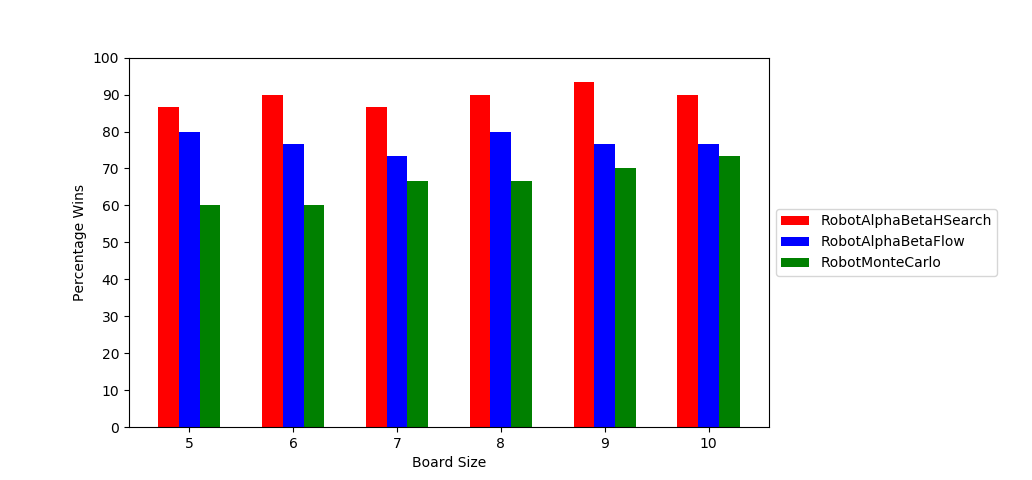
\includegraphics[scale = 0.6]{images/NEWCOMPARISON.png}
    \caption{Effectiveness of various agents against a 4-second per move MCTS agent (no time limit).}
    \label{fig:comparison}
\end{figure}

It is clear to see that the most effective agent in this scenario is RobotAlphaBetaHSearch, shown by the red bars in Figure \ref{fig:comparison}. It consistently had a win-rate above 85\%, and proved to be most effective on larger boards, exhibiting a 93.3\% win-rate on the $9\times9$ board. 


The second most effective agent in this scenario was RobotAlphaBetaFlow, as indicated by the blue bars in Figure \ref{fig:comparison}. It consistently played with a win-rate between 73.3\% and 80\%.

RobotMonteCarlo (indicated by the green line in Figure \ref{fig:comparison}) did not perform as well on smaller sized boards ($5\times5$ to $8\times8$), with a win-rate between 60\% and 66.7\% on these sized boards. This is surprising as this agent is based on the MCTS agent, but with added cell analysis and tree pruning capabilities. However, the agent greatly improves on larger board ($9\times9$ and above), increasing its win-rate to 73.3\%. This is due to inferior cell analysis (with the use of H-Search) having a greater effect on larger boards.














We now consider the effectiveness of the agents when a time limit is imposed. A 60-second time limit will be imposed for each move, which is short enough to highlight the efficiency of each agent, but long enough for each agent to utilize complex algorithms. Figure \ref{fig:comparison2} shows each agent's effectiveness against the same 4-second per move MCTS agent (used in the previous test) with the time limit imposed. 

The results for RobotAlphaBetaHSearch clearly show a reduction in effectiveness on larger boards ($7\times7$ and above), with its win-rate falling below 80\% on $7\times7$ down to 16.7\% on $10\times10$. This is due to the time complexity of the H-Search algorithm. On boards of size $7\times7$ and above, the time required to perform a move exceeds the time allowed, and therefore does not have the time to consider all effective moves, and begins to perform poorly.

Both RobotAlphaBetaFlow and RobotMonteCarlo exhibit similar performance as in the previous test, due to the fact that they are able to decide on a move within the time limit, even for larger boards.




\begin{figure}
    \centering
    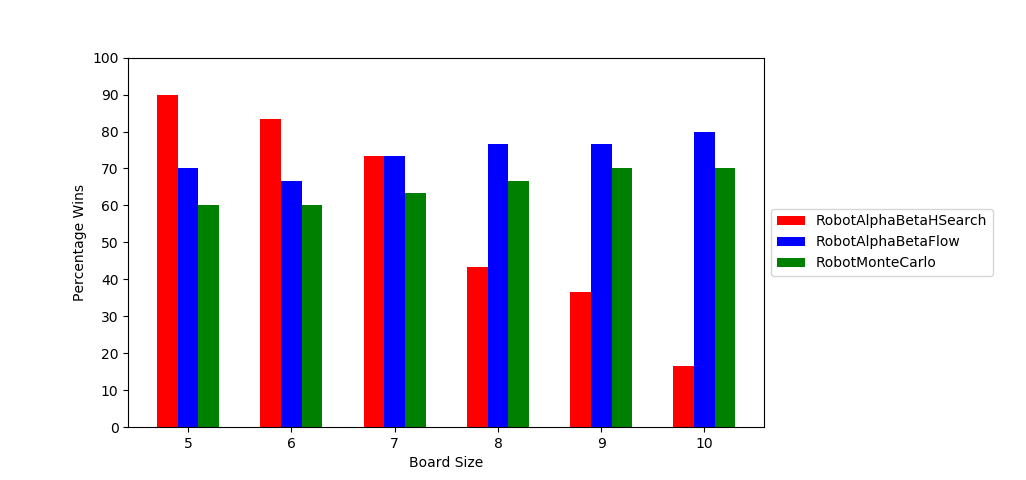
\includegraphics[scale = 0.6]{images/NEWCOMPARISON2.png}
    \caption{Effectiveness of various agents against a 4-second/move MCTS agent (60s time limit).}
    \label{fig:comparison2}
\end{figure}



It is clear that a balance of time allowed and efficacy must be made, particularly from RobotAlphaBetaHSearch. This balance will be different for each agent, so it would be useful to consider their relative performance at varying time allowances, so that we can answer the question of which technique is most successful under a given time restriction. Figure \ref{fig:timecomparison} shows a third experiment to observe each agent's efficacy with various time restrictions. Each agent is played 30 times against a 4-second/move MCTS agent on a $7\times7$ board with various time restrictions, each of which playing first exactly 15 times with the pie rule enabled. It is clear to see that both RobotAlphaBetaFlow and RobotMonteCarlo performed consistently well: with a time limit of 10 seconds and above, RobotMonteCarlo had a win-rate of above 56.7\%, reaching 65-75\% when given at least 30 seconds. RobotAlphaBetaFlow consistently had a win rate of above 70\% when allowed 30 seconds or more to make a move. RobotAlphaBetaHSearch did not perform so well under smaller time restrictions. It was the least effective agent when given less than 70 seconds per move, and had a win-rate of just 13.3\% when allowed 20 seconds per move (less than a third of the win-rate of the other two agents). However, as the time allowed per move increased, its success rose sharply, becoming the (joint) best performing agent when given 70 seconds per move, and far out-performing any other agent with a win rate of above 90\% when given at least 110 seconds per move.


\begin{figure}
    \centering
    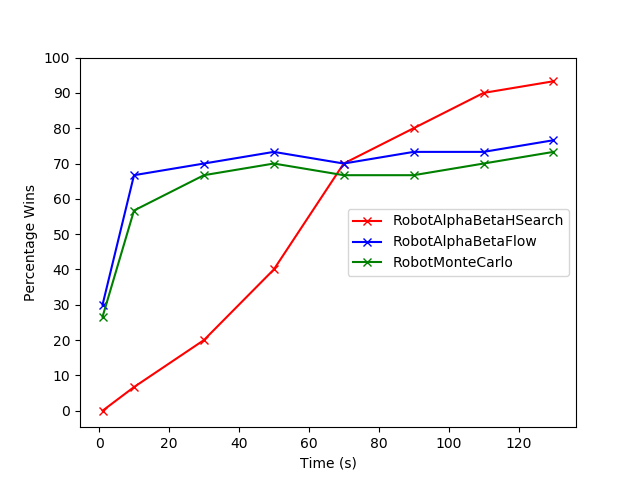
\includegraphics[scale = 0.6]{images/timeComparison.png}
    \caption{Effectiveness of various agents against a 4-second/move MCTS agent.}
    \label{fig:timecomparison}
\end{figure}



















\subsection{Effect of Parameters on Performance}
It is important to see how each agent's parameters affect its performance, both with and without a time restriction. Experiments without a time limit will allow us to see the general trend of the performance according to the parameter, as well as to consider if the parameter is a limiting factor on performance. Experiments with a time limit are made in order to find an optimal value for such a parameter under this time limit. It is important to only change one parameter at a time, so that any difference in performance is known to be from this parameter. Therefore, all parameters will be set to their default setting other than the parameter being evaluated.

We will again test the agents on a $7\times7$ board against a simple MCTS agent with a 4-second per move time restriction which has no inferior cell analysis or tree pruning capabilities.

\subsubsection{RobotAlphaBetaHSearch Parameters}
We start with analysis of RobotAlphaBetaHSearch's parameters, namely depth, M (maximum number of different minimal carriers with the same ends) and K (maximum number of virtual semi-connections on the input side of the \textbf{OR} deduction rule). 



We first consider the depth parameter. With no time restriction, shown in Figure \ref{fig:hsearch_depth_perf} by the red bars, we can clearly see that as depth is increased, a large increase in performance follows, with just a 60\% win-rate for depth of 1 and a 100\% win-rate with a depth of 3. This is clearly because as depth increases, the further minimax will traverse the game tree, allowing for a better understanding of the consequences of playing a particular move and more intelligent play. 



If we now consider the same experiment but with a 60 second time restriction, shown by the blue bars in Figure \ref{fig:hsearch_depth_perf}, it is clear that the best performance is exhibited when depth has a value of 2. The win-rate at this value was 80\%, but drops to 50\% when depth is set to 1, and 30\% when set to 3. When depth is set to 1, the minimax algorithm can only consider the board state after its own move. When depth is set to 3, although the agent performs exceptionally well with no time restriction, the minimax algorithm (along with its complex heuristic) takes a larger amount of time to consider all moves due to its exponential complexity. Therefore, not all moves could be considered, so effectiveness is reduced. Therefore, we conclude that 2 is the most optimal value for the depth parameter.


\begin{figure}
    \centering
    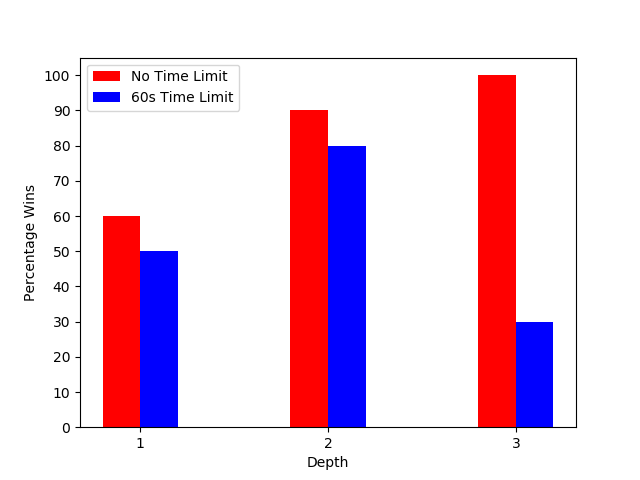
\includegraphics[scale = 0.6]{images/HSEARCHDEPTH_PERF.png}
    \caption{The effect of the depth value on RobotAlphaBetaHSearch against a 4-second/move MCTS agent.}
    \label{fig:hsearch_depth_perf}
\end{figure}
















Now we can analyze the effect of parameter M on the performance of RobotAlphaBetaHSearch. Firstly, we shall consider the experiment with no time limit, shown by the red bars in Figure \ref{fig:hsearch_m_perf}. The M value exhibits poor performance at smaller values. With M equal to 0, the agent is playing with no virtual connections, since no carriers are allowed for any virtual connection. Therefore, the heuristic function is very weak as it cannot use any advantage that H-Search brings. This is supported by the poor win-rate of 20\%. Beyond a value of 0, the performance increases to a win-rate of 70\% when M is 4, and a win-rate of 90\% when M is 12. Beyond this value, there is little change in effectiveness. This is most likely due to the fact that on a $7\times7$ board, virtual connections do not generally have more than 10-12 different minimal carriers. Therefore, increasing M has little effect on performance. 

Imposing a 60 second time limit changes the results, especially for larger values of M, shown by the blue bars in Figure \ref{fig:hsearch_m_perf}. The effectiveness closely matches that from the previous experiment for M values up to 8, with the win-rate reaching 70\% for M equal to 10, but for M larger than 12 we see a decline in performance down to a 50\% win-rate for M equal to 20. As M increases, there is potential for more carriers to be stored, so H-Search may have more virtual connections to generate which will increase running time. Therefore, the time required per move may start to exceed the time allowed, reducing the effectiveness of the agent. This is precisely what is seen in the results of this experiment, which allows us to therefore conclude that the optimal value of M is between 8 and 12, as this is what gave the highest win-rate under this time restriction.

\begin{figure}
    \centering
    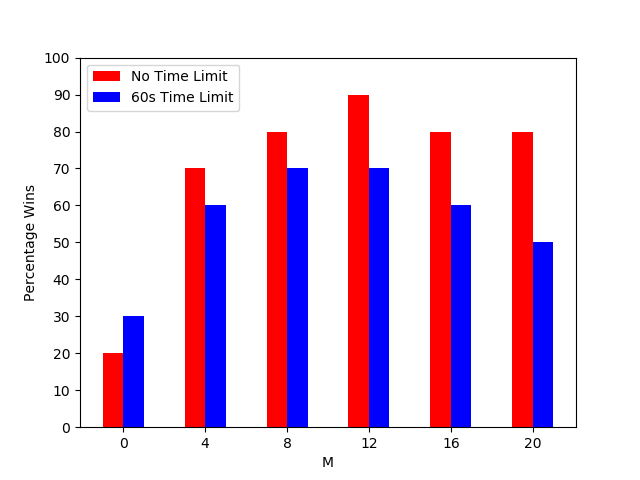
\includegraphics[scale = 0.6]{images/HSEARCHM_PERF.png}
    \caption{The effect of the M value on RobotAlphaBetaHSearch against a 4-second/move MCTS agent.}
    \label{fig:hsearch_m_perf}
\end{figure}










The last parameter of RobotAlphaBetaHSearch we will analyze is K. The red bars in Figure \ref{fig:hsearch_k_perf} shows how the agent's win-rate changes with respect to the value of K. It is very clear to see that the relationship between K and the agent's effectiveness is close to linear: as K increases, the win-rate also increases (at a near constant rate) until k is equal to 5, at which the win-rate is 100\%. The agent performs poorly for lower values of K, with just a 30\% win-rate at K equal to 0. This is easily explainable through the implementation of the \textbf{OR} deduction rule. When K is 0, the algorithm does not take any carriers of virtual semi-connections as an input. Therefore, the algorithm will not build any virtual connections through the deduction rule. We are only left with the initial virtual connections between adjacent cells. This means the algorithm cannot make use of H-Search to the fullest extent. The agent clearly gets more effective as K increases, due to the fact that more complex virtual connections can be made through the \textbf{OR} deduction rule if more virtual semi-connections are used as an input.

Now considering the result of the experiment under a 60 second time restriction, shown by the blue bars in Figure \ref{fig:hsearch_k_perf}, we can see that the effectiveness is optimal when K is equal to 3. After this value, the time spent using the \textbf{OR} deduction rule becomes so large that the agent cannot consider all moves, rendering it less effective. This is due to the exponential time complexity of the deduction rule. We conclude that the optimal value of the K parameter is 3, where the efficacy of the agent peaks in Figure \ref{fig:hsearch_k_perf}.



\begin{figure}
    \centering
    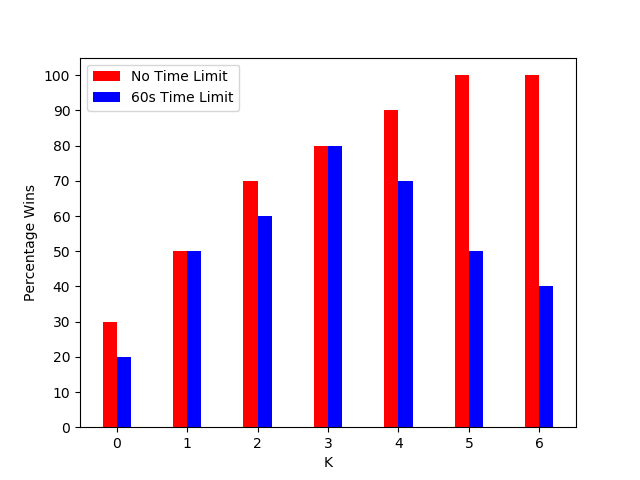
\includegraphics[scale = 0.6]{images/HSEARCHK_PERF.png}
    \caption{The effect of the K value on RobotAlphaBetaHSearch against a 4-second/move MCTS agent.}
    \label{fig:hsearch_k_perf}
\end{figure}









\subsubsection{RobotAlphaBetaFlow Parameters}

RobotAlphaBetaFlow has just one parameter, depth. This is again used to set the maximum depth of the game tree in the minimax algorithm.

Figure \ref{fig:flowdepth_perf} shows the affect of the value of depth on RobotAlphaFlowNetwok's performance. The red bars show the effect of the value on performance with no time restraint. Here we can see that the agent's effectiveness increases with depth, starting at 50\% with a depth of 1 up to 90\% with a depth of 4. This is a huge gain of performance, but since the size of the game tree is exponential in depth, it is not surprising.

The blue bars in Figure \ref{fig:flowdepth_perf} show the effect on performance with a time limit of 20 seconds per move. Here we see the performance closely matches that of the previous results for depth less than 4, but for depth equal to 4 performance is reduced. As depth increases, we see an increase in the running time of the minimax algorithm, and depth 4 seems to be where the algorithm takes a time greater than the time limit, thus reducing performance. Here we conclude that 3 is the optimal value of depth for games with this time limit.

\begin{figure}
    \centering
    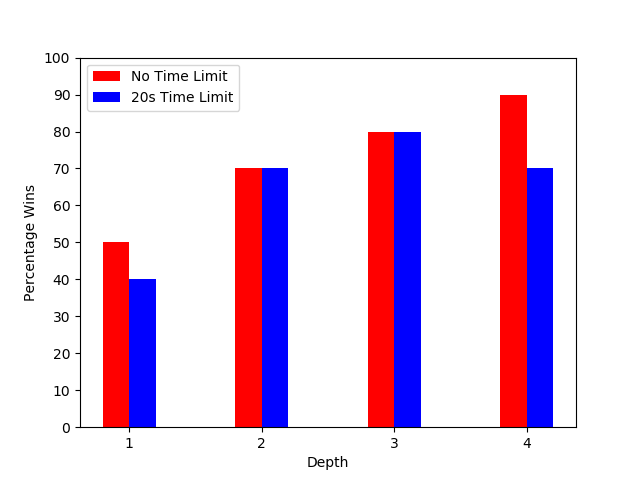
\includegraphics[scale = 0.6]{images/FLOWDEPTH_PERF.png}
    \caption{The effect of the depth value on RobotAlphaBetaFlow against a 4-second/move MCTS agent.}
    \label{fig:flowdepth_perf}
\end{figure}



\subsubsection{RobotMonteCarlo Parameters}




Finally we analyze the effect of RobotMonteCarlo's parameters on performance, namely MCTS-time, win-score and knowledge-threshold.

As we increase the amount of time that the tree search in RobotMonteCarlo has to simulate playouts and build its game tree, the more successful we expect the agent to be at playing against the 4-second per move MCTS agent. This certainly is the case, illustrated in Figure \ref{fig:mctime_perf}. It is clear to see that the effectiveness is extremely poor at MCTS-Time equal to 0, with a win-rate of just 10\%. This makes sense, since with no time to run MCTS the agent plays randomly, and thus poorly, against the agent. The agent reaches a win-rate of 60\% at MCTS-Time equal to 4 seconds, matching the time allowed for the opposing agent. It is due to the cell analysis and tree pruning capabilities of RobotMonteCarlo that makes the agent have a win-rate greater than 50\% against the opposing agent which also uses MCTS. The agent eventually plateaus at a 60 - 70\% win-rate from a value of 5 seconds and longer. 



\begin{figure}
    \centering
    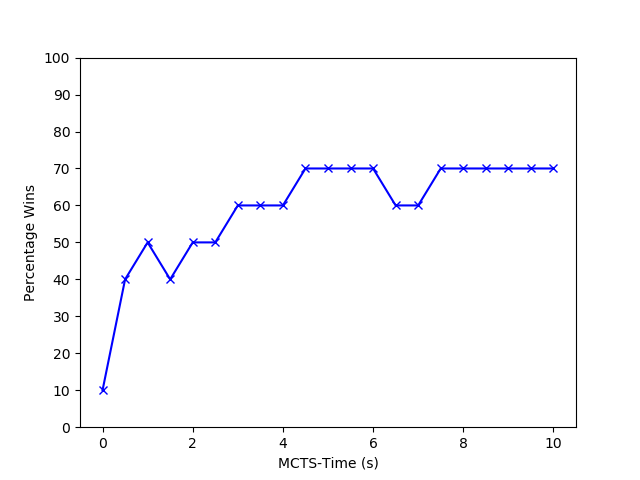
\includegraphics[scale = 0.6]{images/MCTIME_PERF.png}
    \caption{The effect of the MCTS-Time value on RobotMonteCarlo against a 4-second/move MCTS agent.}
    \label{fig:mctime_perf}
\end{figure}










When experimenting with different values of the knowledge-threshold, it is important to consider the performance of the agent when time is not a factor, as this is another parameter that impacts performance. Hence, we allow MCTS to perform a set number of iterations (10,000) to enable the agent to fully use any cell analysis technique that may otherwise take up time. This is clearly illustrated in Figure \ref{fig:mcknowledge_perf} by the red bars. With a knowledge-threshold of 0, we perform cell analysis for every node. This greatly increases the effectiveness of the agent, with a 100\% win-rate. As the knowledge-threshold is increased, we perform cell analysis for less nodes, which is shown to reduce the performance, down to a 70\% win-rate at a knowledge-threshold of 60.

When a time limit of 20 seconds was imposed, the results changed substantially, shown in Figure \ref{fig:mcknowledge_perf} by the blue bars. When the knowledge-threshold was set to 0, it was found that the win-rate was very poor at just 20\%. This is due to the algorithm spending a very large proportion of time performing cell analysis and not expanding the game tree. In this case the algorithm had a very clear understanding of the value of the board states it did consider, but did not have this understanding of more than a handful of states. Therefore, its selection of moves was limited. As the knowledge-threshold was raised to values between 20 and 30, the win-rate increased to 80\%, which was the highest recorded in this experiment (with the time restriction). After this, however, the win-rate reduced to 60-70\% with a knowledge-threshold of 40-60. This is due to the algorithm performing cell analysis on too few nodes, which does not allow for the fullest use of the analysis. We can conclude that the optimal value of knowledge-threshold is approximately 25.


\begin{figure}
    \centering
    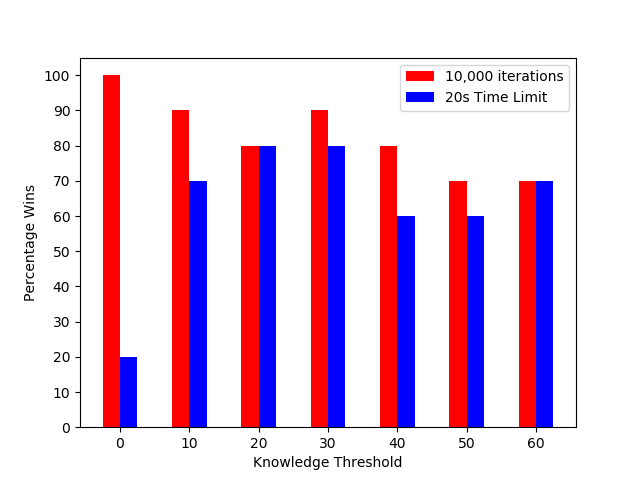
\includegraphics[scale = 0.6]{images/MCKNOWLEDGE_PERF.png}
    \caption{The effect of the knowledge-threshold value on RobotMonteCarlo against a 4-second/move MCTS agent.}
    \label{fig:mcknowledge_perf}
\end{figure}







RobotMonteCarlo's final parameter, win-score, is a parameter that theoretically should not impact performance (for values above 0). This was confirmed in the experiment (with not time restriction) shown in Figure \ref{fig:mcwin_perf}, which shows the the agent had a win-rate of 60-70\% for win-score values of greater than 0. This is simply because the win-score is a constant value, of which its value makes no difference, so long as it is constant (and positive). When win-score was set to 0, the agent showed poor performance (win-rate of 20\%). This is because there is no way of keeping track of which nodes in the game tree are successful, so the agent exhibits random behaviour.
\begin{figure}
    \centering
    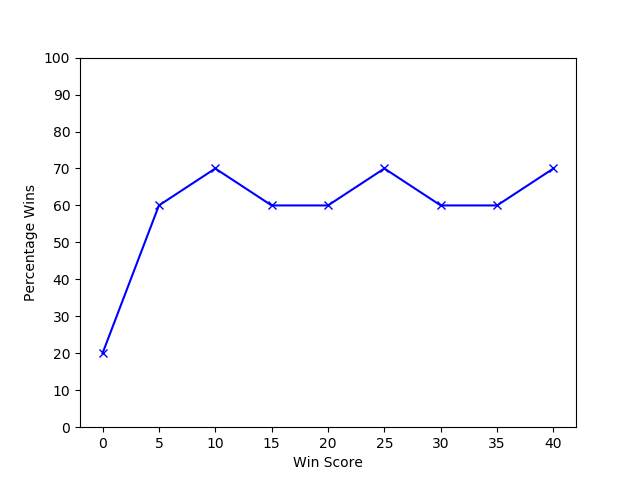
\includegraphics[scale = 0.6]{images/MCWIN_PERF.png}
    \caption{The effect of the win-score value on RobotMonteCarlo against a 4-second/move MCTS agent}
    \label{fig:mcwin_perf}
\end{figure}





\subsection{Effect of Parameters on Efficiency}
Another important consequence of the parameter settings to analyze is their impact on the running time of the agent (the time required to make a single move). Experiments in this section are conducted in the following way: each parameter will be set to a number of different values (with every other parameter set to its default value), and the time the agent takes to choose the first move (playing first, with the pie rule enabled) is recorded. The experiment is conducted three times, and the average time is calculated for various values of the parameter.



\subsubsection{RobotAlphaBetaHSearch Parameters}
We start with RobotAlphaBetaHSearch. The data recorded for the depth parameter's effect on efficiency can be seen in Figure \ref{fig:hsearch_depth_time}. It is clear that the relationship between depth and the time required per move exhibits an exponential relationship. This is not at all surprising, since the size of the game tree is exponential in depth. On a $7\times 7$ board, the branching factor is $7^2 = 49$ for an empty board, so we would expect the time taken for depth \textit{d} to be approximately 50 times greater than the time taken for depth \textit{d-1}. This is not quite reflected in Figure \ref{fig:hsearch_depth_time}: when depth is 2, the time required is around 75 seconds, whereas when depth is 3, the time required only increases to around 615 seconds (less than a factor of 10 increase). This may be because the effect of various pruning techniques in this agent become greater at higher depths. For example, more information about the opponent's virtual connections is found after more moves have been played, so less moves are considered (the agent does not consider attacking an opponent's virtual connection as this is useless). Alpha-beta pruning also has an increase in effectiveness as depth increases.

\begin{figure}
    \centering
    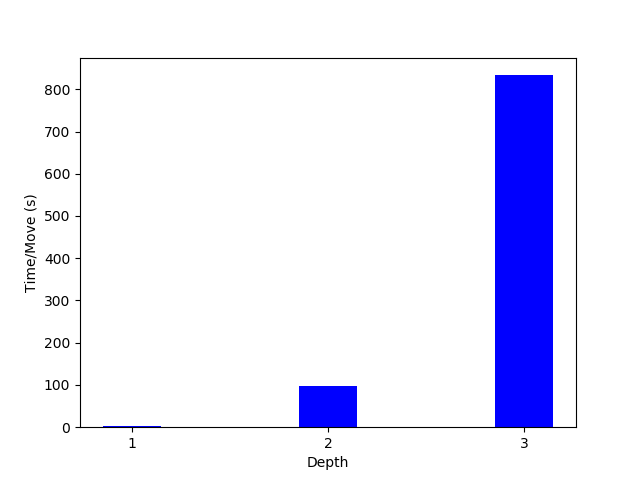
\includegraphics[scale = 0.6]{images/HSEARCHDEPTH_TIME_INF.png}
    \caption{The effect of the depth value on the efficiency of RobotAlphaBetaHSearch.}
    \label{fig:hsearch_depth_time}
\end{figure}













We now consider the impact of the parameters M and K on the time required per move. As described before, M is the maximum number of different minimal carriers for each virtual connection, and K is the maximum number of virtual semi-connections on the input side of the \textbf{OR} deduction rule. The effect of M and K on time required per move can be seen in Figures \ref{fig:hsearch_m_time} and \ref{fig:hsearch_k_time} respectively. 

As M increases, the time required per move by the agent increases steadily, reaching around 140 seconds with a value of 25. With more carriers between each pair of ends to maintain, more time is used to build up other virtual connections, thus greatly increasing the complexity of the algorithm. Towards larger values of M, however, we see a slight taper in the time needed. This is because there are simply no more carriers to be found between the majority of ends.

It is clearly shown that K has a notable effect on the time required per move, with the time required for K equal to 8 being almost 10 times greater than for K equal to 0; there is a sharp increase from 20 seconds at K equal to 0, up to 200 seconds with K equal to 8. This is explained by the recursive nature of the implementation of the \textbf{OR} deduction rule:

The \textbf{OR} rule is applied during the consideration of the two ends g1 and g2, and a midpoint g, when we have found two sets c1 and c2 such that $c1 \cap c2 = \empyset$, and $g1 \notin c2$ and $g2 \notin c1$. The implementation of this rule works by taking a set of carriers (of virtual semi-connections) between two ends as an input. Two other sets, \textbf{UNION} and \textbf{INTERSECTION} are maintained, having been initialized to both be $c1 \cup \{g\} \cup c2$. It then loops over each carrier (of a virtual semi-connection) and either recursively calls the \textbf{OR} deduction rule, updating \textbf{UNION} to include the carrier, and \textbf{INTERSECTION} to be reduced to those also in the carrier, or we terminate (if \textbf{INTERSECTION} is empty). The time complexity of this rule is exponential in the size of the set of carriers, so it is not surprising that K exhibits such an effect on the time required per move.

\begin{figure}
    \centering
    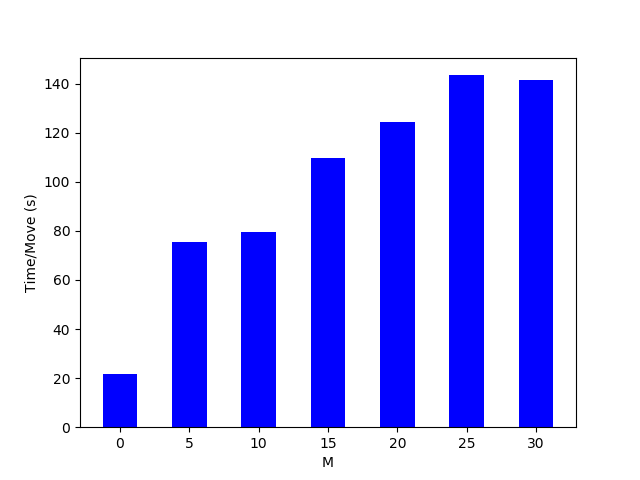
\includegraphics[scale = 0.6]{images/HSEARCHM_TIME_INF.png}
    \caption{The effect of the M value on the efficiency of RobotAlphaBetaHSearch.}
    \label{fig:hsearch_m_time}
\end{figure}

\begin{figure}
    \centering
    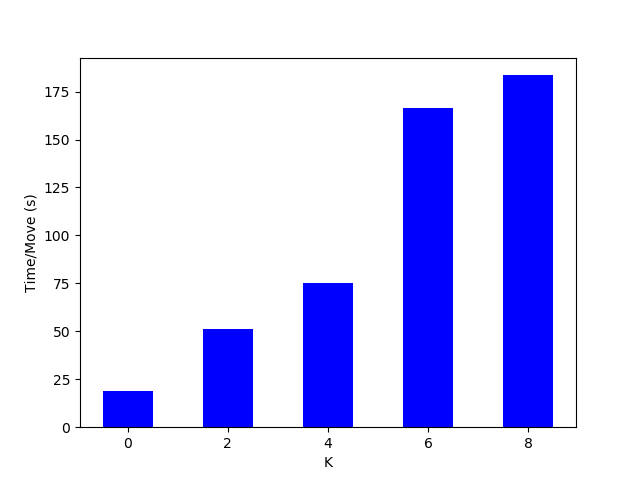
\includegraphics[scale = 0.6]{images/HSEARCHK_TIME_INF.png}
    \caption{The effect of the K value on the efficiency of RobotAlphaBetaHSearch.}
    \label{fig:hsearch_k_time}
\end{figure}






\subsubsection{RobotAlphaBetaFlow Parameters}
Now we evaluate the effect of the parameter in RobotAlphaBetaFlow, depth. The results (shown in Figure \ref{fig:flow_depth_time}) clearly indicate that depth has a large impact on the time required per move: for a depth of 3, 28 seconds is required, but a depth of 4 increases this to over 60 seconds. However, the same phenomenon can be seen as in Figure \ref{fig:hsearch_depth_time}, where a higher proportion of time is saved using optimization techniques at higher values of depth, leading to a shallower graph. In RobotAlphaBetaFlow, the implementation makes use of previously made flow networks to avoid redundantly recreating them. The effect on efficiency is more noticeable at higher levels of depth. 


\begin{figure}
    \centering
    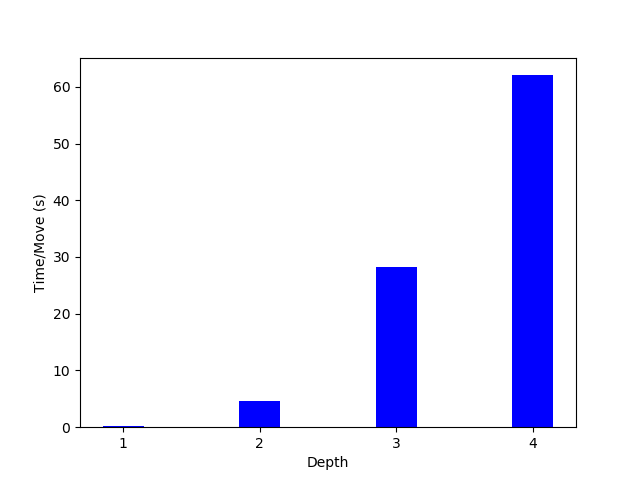
\includegraphics[scale = 0.6]{images/FLOWDEPTH_TIME_INF.png}
    \caption{The effect of the depth value on the efficiency of RobotAlphaBetaFlow.}
    \label{fig:flow_depth_time}
\end{figure}


\subsubsection{RobotMonteCarlo Parameters}
We now evaluate RobotMonteCarlo's parameters. RobotMonteCarlo has three parameters: MCTS-Time, win-score and knowledge-threshold. There is no need to analyze the time required for different values of win-score as this parameter does not impact complexity in any way. There is also no need to run this experiment for MCTS-Time, since this variable directly controls the amount of time allowed, so performing this experiment is useless.



We analyze the effect of the knowledge-threshold on the time required per move. We must not fix the amount of time allowed for MCTS, as this would defeat the point of this experiment. Instead, a fixed number of iterations will be used to avoid making any restriction on time. In this particular experiment, 10,000 iterations was used. Figure \ref{fig:mc_knowledge_time} shows that increasing the threshold generally leads to less time required per move. This makes sense, since a higher threshold implies a lower number of nodes that inferior cell analysis is performed on. This analysis is very costly, as it makes use of the H-Search algorithm.   
\begin{figure}
    \centering
    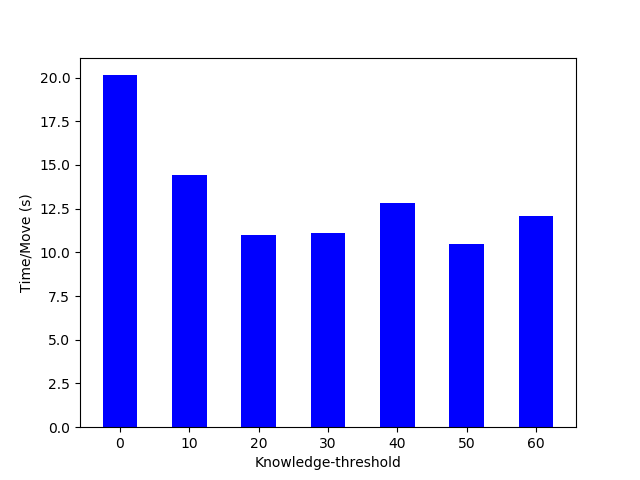
\includegraphics[scale = 0.6]{images/MCKNOWLEDGE_TIME_INF.png}
    \caption{The effect of the knowledge-threshold value on the efficiency of RobotMonteCarlo with 10,000 iterations.}
    \label{fig:mc_knowledge_time}
\end{figure}